\hypertarget{the-flyer}{%
\section{\texorpdfstring{\href{https://canva.link/nq5h2a1emeity4d}{The
Flyer}}{The Flyer}}\label{the-flyer}}

For this activity, I created a flyer targeted toward seniors. It
provides some general guidelines on staying safe online (which is
information many seniors will not know), including 3 tips (using secure
passwords, reading communication carefully, and ensuring that HTTPS is
being used) and 3 places to report scams to (Scamwatch, ACSC, and WA
ScamNet).

\begin{figure}
\centering
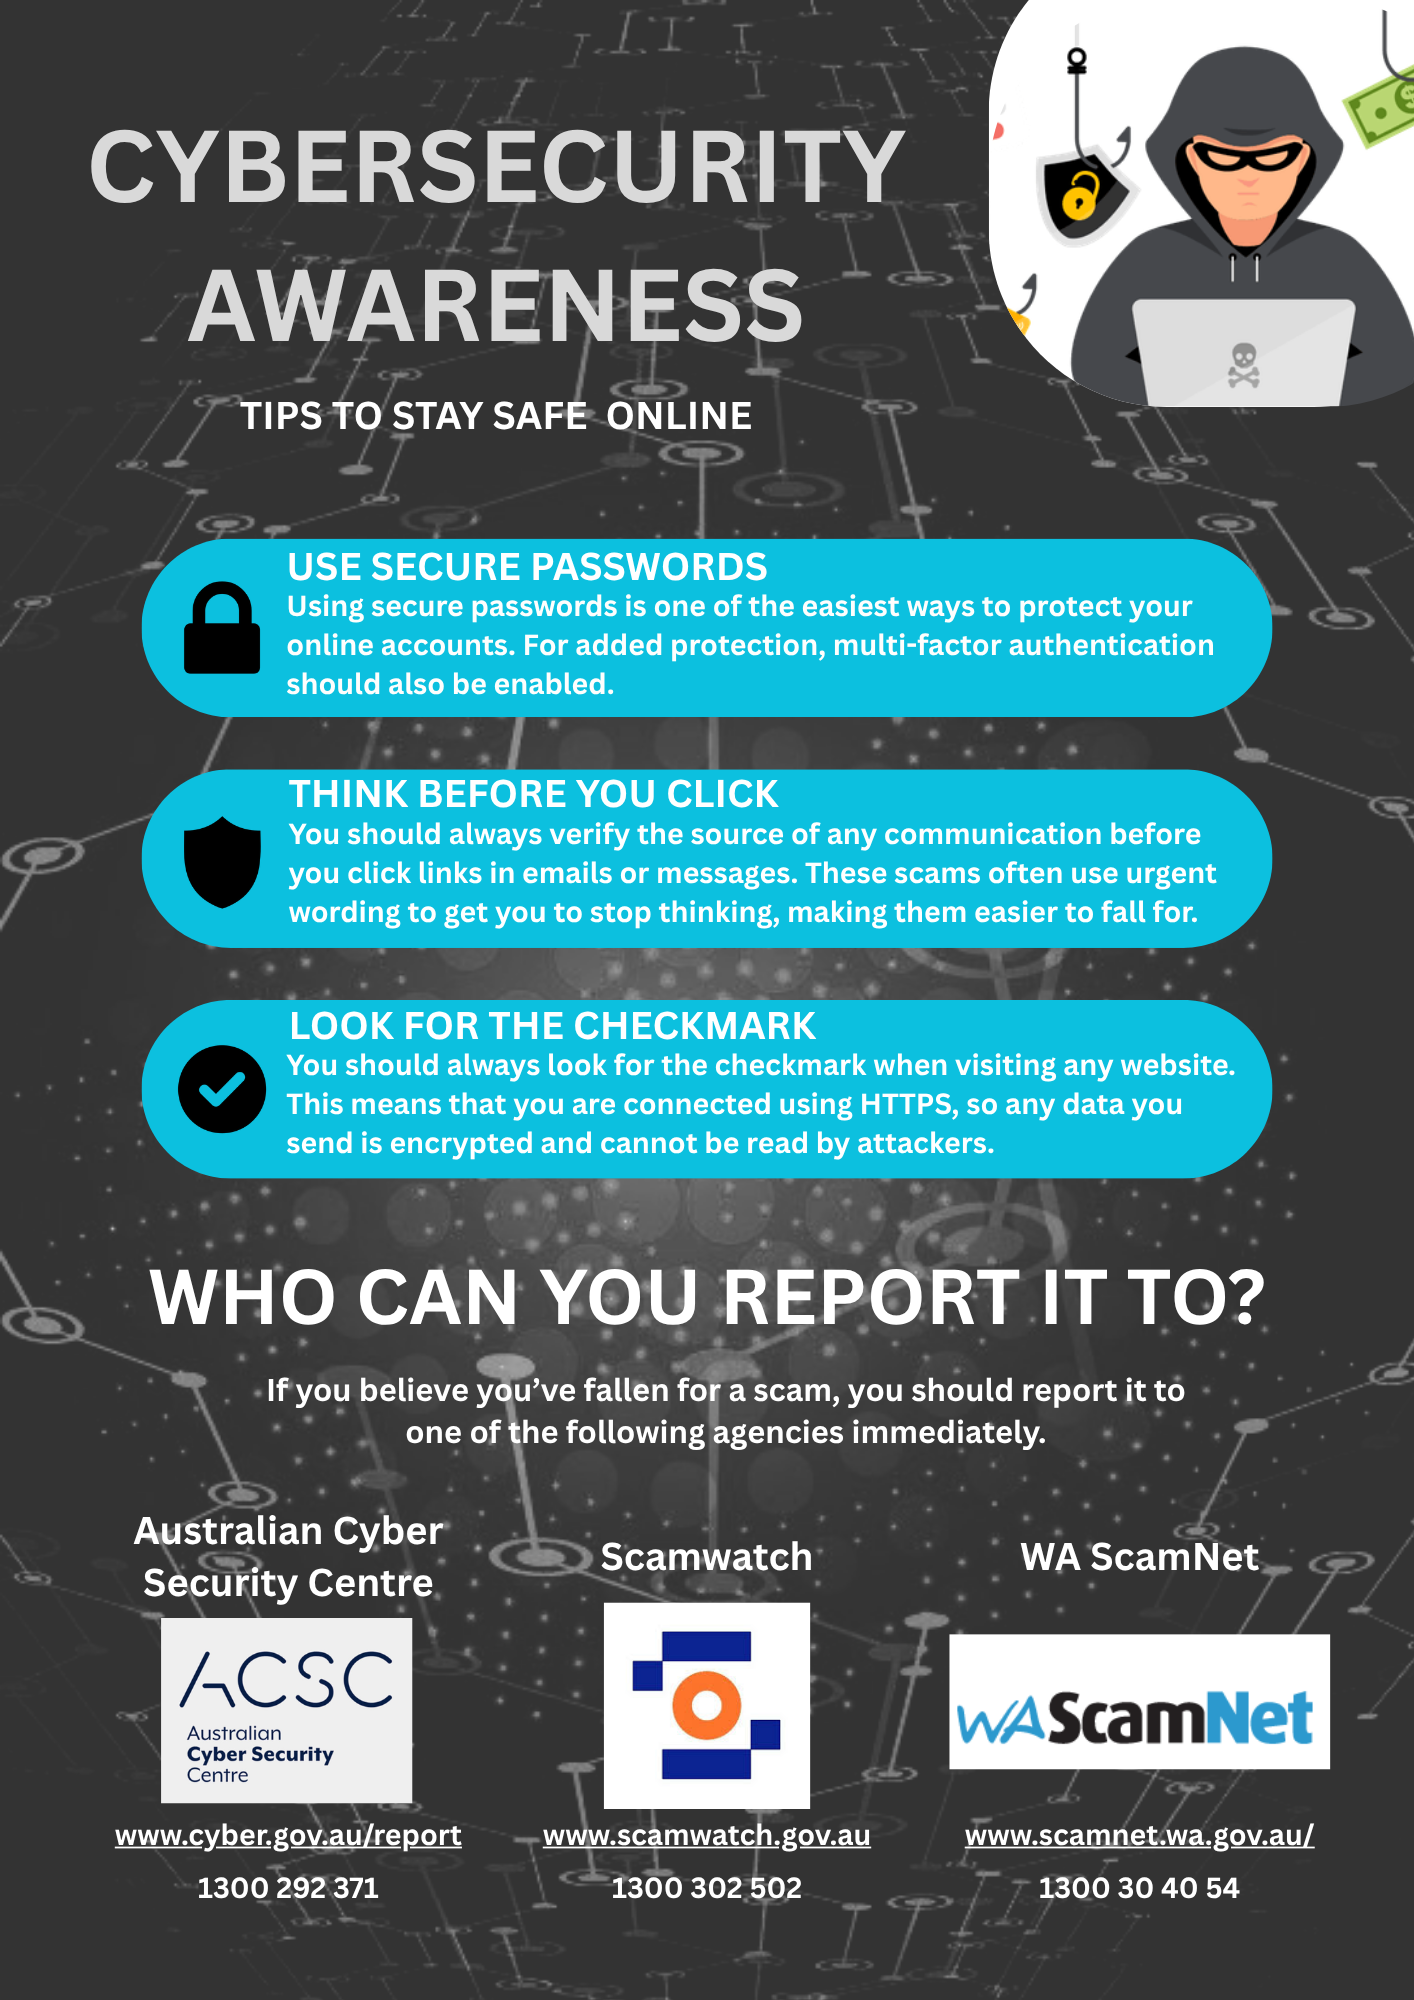
\includegraphics{flyer.png}
\caption{flyer}
\end{figure}

\hypertarget{references}{%
\section{References}\label{references}}

Freedesignfile. ``Virtual technology line background vector 02''.
Accessed: May 12, 2026. {[}Online{]}. Available:
https://freedesignfile.com/510008-virtual-technology-line-background-vector-02/

Firstrust Bank. '' TAKING ACTION AGAINST FRAUD \& SCAMS''. Accessed: May
12, 2026. {[}Online{]}. Available:
https://www.firstrust.com/security-first

D. Gandy. ``Padlock free icon''. Accessed: May 12, 2026. {[}Online{]}.
Available: https://www.flaticon.com/free-icon/padlock\_25239

Freepik Company S.L.U. ``Computer Security Shield free icon''. Accessed:
May 12, 2026. {[}Online{]}. Available:
https://www.flaticon.com/free-icon/computer-security-shield\_74662

meaicon. ``Check free icon''. Accessed: May 12, 2026. {[}Online{]}.
Available: https://www.flaticon.com/free-icon/check\_17767109
